\section{Static Design Phase}
\label{sec:static_system}
The system described in this paper operates in two phases.
The first phase relies on Vivado to create an initial static design and the second phase, the Maverick flow, allows the creation of subsequent RMs, independent of Vivado.
This section describes that first phase, the static design phase.

As shown in \figurename~\ref{fig:static_system}, this phase is made up of three steps to create the full static design.
The full static design consists of a Vivado-generated static design, containing a static region and a PR region, and some associated metadata.
This metadata describes the PR region and its interface with the static region.

\begin{figure}
	\centering
	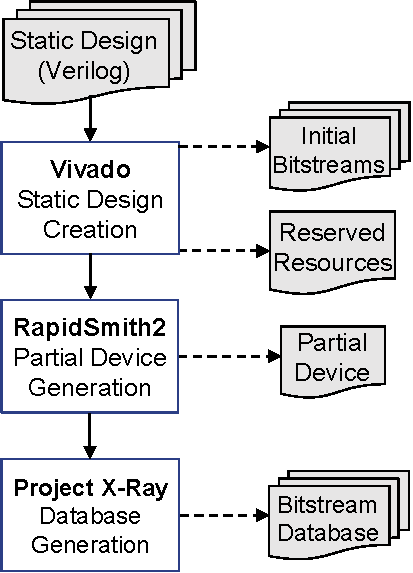
\includegraphics[height=.68\columnwidth]{figures/static_system.pdf}
	\caption{Static Design Phase}
	\label{fig:static_system}
\end{figure}

\subsection{Static Design Creation: Vivado}
In the first step of the static design phase, a base static design is created and compiled using Vivado's PR flow.
First, the static design HDL, which contains static logic and a black box RM, is synthesized with Vivado's PR flow. 
An initial RM HDL design is then separately synthesized with Vivado's PR flow.

Next, a floorplan is created to define the PR region into which RMs will be physically implemented.
This PR region must be chosen to adhere to certain horizontal and vertical alignment requirements imposed by the device architecture \cite{Xilinx:2018d}.
The initial synthesized RM design is then assigned to this PR region, creating an initial full-device design.

\begin{figure}
	\centering
	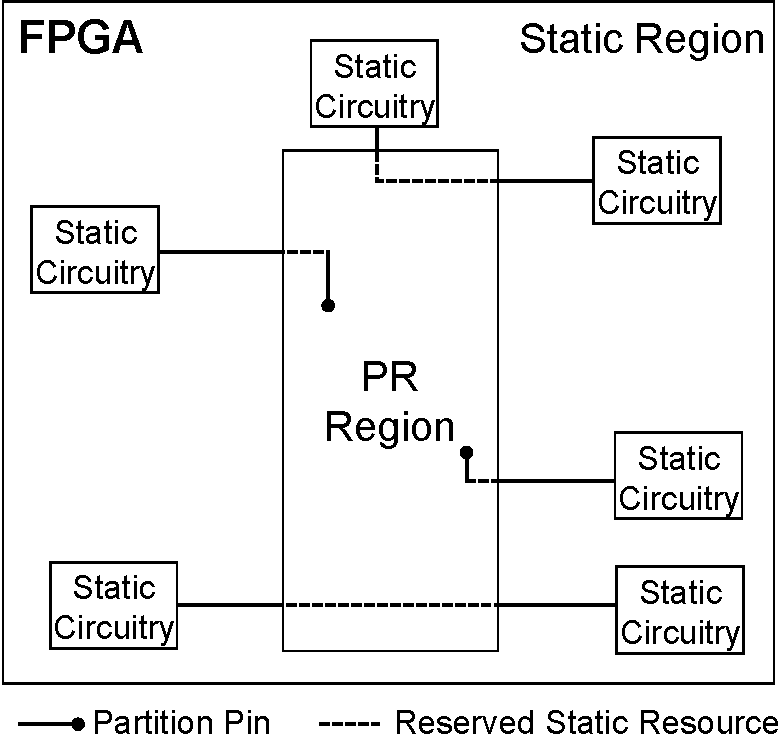
\includegraphics[width=.65\columnwidth]{figures/partPins.pdf}
	\caption{A Static Design with Partition Pins and Reserved Resources}
	\label{fig:partPins}
\end{figure}

Vivado's PR flow is then used to place and route this full-device design.
All static logic is constrained to be within the static region of the FPGA, while RM logic is constrained to be within the PR region.
However, some routing resources within the PR region may be used to route static circuitry; these resources are reserved by the static design and cannot be used by RMs.
\figurename~\ref{fig:partPins} shows a static design and represents these reserved routing resources as dashed lines.

Placement and routing also results in the creation of partition pins, which are the logical and physical points at which the static logic and RMs interface.
These partition pins act as top-level ports for the RM designs implemented within the PR region, giving the RM designs access to I/O and other global resources located in the static region.
Partition pins are physically implemented as wire segments within PR regions \cite{Xilinx:2018d}.
Vivado's PR flow creates routes that connect the static logic and the partition pins, as seen in \figurename~\ref{fig:partPins}.
These partition pins and routes are also reserved by the static design and must be consistent across all RMs.

After Vivado's PR flow finishes creating the static design, a bitstream corresponding to the static (base) part of the design is generated; this can be used to pre-configure the FPGA prior to any partial bitstreams being configured onto it.
Next, an initial partial bitstream corresponding to the empty PR region, containing no RM circuitry, is created.
Custom Tcl scripts are then executed within Vivado to generate a list of routing resources that are reserved by the static design and which lie within the PR region.
The Maverick flow needs this list to prevent these resources from being used during the RM implementation stages.
These two pieces of data (bitstreams and reserved resources) are shown in the upper right portion of \figurename~\ref{fig:static_system}.

\subsection{Partial Device Model: RapidSmith2}
RapidSmith2 \cite{Haroldsen:2015} is an open-source FPGA CAD tool framework which provides a design representation and a circuit manipulation API upon which CAD tools can be written. 
The next step in the static design phase is the creation of a {\em partial device model}, which is used by the RapidSmith2-based tools of the Maverick flow.
RapidSmith2 normally creates full device models for its own use by parsing XDLRC files, which describe Xilinx device data in great detail.
For modern Xilinx devices, these XDLRC files are generated using Tincr \cite{White:2014} and the Vivado Design Interface (VDI) \cite{Townsend:2017b}, which together contain a library of Tcl and Java routines to enable the export and import of device and design data.

To create partial device models, a new RapidSmith2-based partial device generator is used.
This partial device model describes only the resources within a specified PR region of a device that are available to the Maverick flow for implementing RM designs.
This includes all the logic slices, clocking resources, interconnect, and other configurable resources within the PR region.
Additionally, this model describes all interconnect resources that can be used to enter or leave the PR region.
Because this partial device model describes only a particular subset of the full FPGA (i.e., the PR region), the memory required to represent the design is greatly reduced.

\subsection{Bitstream Database Generation: Project X-Ray}
The last set of static design metadata that needs to be generated is a Project X-Ray \cite{PrjXray} bitstream database.
Project X-Ray is an open-source project that aims to document the Xilinx 7-Series bitstream format.
Project X-Ray does this by using Vivado's Tcl API to generate bitstreams for several small designs with specific properties.
Several tools are then used to analyze these bitstreams and to map specific device features to specific bits in the bitstream, resulting in a bitstream database.

At the time of the writing of this paper, Project X-Ray generates a bitstream database for a subset of 7-Series device features within a specific region of interest in an Artix7 FPGA.
As a part of our work, we modified several of the Project X-Ray Tcl scripts to support Zynq FPGAs.
This bitstream database in conjunction with the initial partial bitstream (created with Vivado's PR flow) provides the necessary information for the Maverick flow to generate new partial bitstreams for placed and routed designs within the PR region.
At this point, the static design phase is complete and Vivado is no longer needed.
